
%%%%%%%%%%%%%%%%% - GLOSARIO - %%%%%%%%%%%%%%%%%%%

% -------------------- 0 - 9 ------------------- %

\newglossaryentry{3dgaussiansplatting}
{
    name={\acrshort{3d} Gaussian Splatting},
    description={TBD. ver seción tal de herramientas. citar paper}
}

% ---------------------- A --------------------- %

\newglossaryentry{actor}
{
    name={actor},
    description={Desambiguación. En \gls{unrealengine}... TBD}
}

\newglossaryentry{actores}
{
    name={actores},
    description={. Ver \gls{actor}}
}

% ---------------------- B --------------------- %

\newglossaryentry{blender}
{
    name={Blender},
    description={TBD. ver seción tal de herramientas}
}

\newglossaryentry{blueprint}
{
    name={blueprint},
    description={En \gls{unrealengine}... TBD}
}

% ---------------------- C --------------------- %

\newglossaryentry{client}
{
    name={client},
    description={ver \gls{cliente}}
}

\newglossaryentry{cliente}
{
    name={cliente},
    description={TBD}
}

\newglossaryentry{colmap}
{
    name={COLMAP},
    description={TBD. ver seción tal de herramientas}
}

\newglossaryentry{cpp}
{
    name={C++},
    description={TBD}
}

\newglossaryentry{cudarchitecture}
{
    name={Compute Unified Device Architecture},
    description={o Arquitectura Unificada de Dispositivos de Cómputo}
}

\newglossaryentry{cuda-samples}
{
    name={cuda-samples},
    description={TBD}
}

% ---------------------- D --------------------- %

\newglossaryentry{datacenter}
{
    name={datacenter},
    description={TBD}
}

\newglossaryentry{dataset}
{
    name={dataset},
    description={TBD}
}

\newglossaryentry{debug}
{
    name={debug},
    description={TBD}
}

\newglossaryentry{digitaltwin}
{
    name={Digital Twin},
    description={o gemelo digital es una representación digital de un objeto, generalmente un \gls{modelo3d}. En robótica y automatización se usa para realizar versiones virtuales de robots o máquinas para simular su funcionamiento antes de su puesta en marcha o durante su operación.}
}

% ---------------------- E --------------------- %

% ---------------------- F --------------------- %

\newglossaryentry{ffmpeg}
{
    name={FFmpeg},
    description={TBD. ver seción tal de herramientas}
}

\newglossaryentry{fotogrametria}
{
    name={fotogrametría},
    description={es el método destinado a analizar y determinar con exactitud la geometría, tamaño y ubicación espacial de un objeto, empleando principalmente mediciones realizadas a partir de una o más imágenes fotográficas de dicho objeto.}
}

\newglossaryentry{funcionplenoptica}
{
    name={función plenóptica},
    description={TBD: traducir. ``Consider, first, a black and white photograph taken by a pinhole camera. It tells us the intensity of light seen from a single viewpoint, at a single time, averaged over the wavelengths of the visible spectrum. That is to say, it records the intensity distribution $P$ within the pencil of light rays passing through the lens. This distribution may be parameterized by the spherical coordinates, $P(\theta,\phi)$, or by the Cartesian coordinates of a picture plane, $P(x,y)$ (figure 1.2; see discussion below). A color photograph adds some information about how the intensity vanes with wavelength $\lambda$, thus: $P(\theta,\phi,\lambda)$. A color movie further extends the information to include the time dimension $t$: $P(\theta,\phi,\lambda,t)$. A color holographic movie, finally, indicates the observable light intensity at every viewing position, $V_x$, $V_y$, and $V_z$: $P(\theta,\phi,\lambda,t,V_x,V_y,V_z)$. A true holographic movie would allow reconstruction of every possible view, at every moment, from every position, at every wavelength, within the bounds of the space-timewavelength region under consideration. The plenoptic functions is equivalent to this complete holographic representation of the visual world.
    \begin{figure}[H]
        \centering
        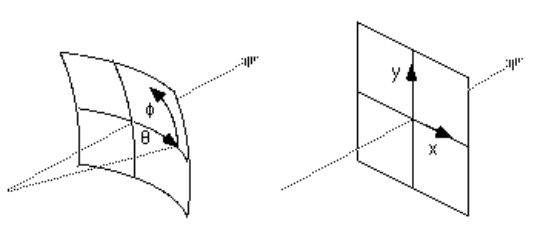
\includegraphics[scale=0.5]{imagenes/funcion-plenoptica/funcion-plenoptica.png}
        \caption{The image information available from a single viewing position is defined by the pencil of light rays passing through the pupil. The rays may be parameterized in angular coordinates or in Cartesian coordinates. The Cartesian approach is commonly used in machine vision and computer graphics, but the angular approach can more easily represent the full sphere of optical information impinging on a point in space.}
        \label{fig:funcion-plenoptica}
    \end{figure}
    Such a complete representation would contain, implicitly, a description of every possible photograph that could be taken of a particular space-time chunk of the world (neglecting the polarization and instantaneous phase of the incoming light)"}
}

% ---------------------- G --------------------- %

\newglossaryentry{gemelodigital}
{
    name={gemelo digital},
    description={TBD. ver \gls{digitaltwin}}
}

\newglossaryentry{github}
{
    name={GitHub},
    description={TBD}
}

% ---------------------- H --------------------- %

\newglossaryentry{hardware}
{
    name={hardware},
    description={TBD}
}

\newglossaryentry{hierarchicallocalization}
{
    name={Hierarchical Localization},
    description={TBD. \cite{sarlin2019coarse}}
}

\newglossaryentry{host}
{
    name={host},
    description={TBD}
}

% ---------------------- I --------------------- %

\newglossaryentry{inputmappingcontext}
{
    name={Input Mapping Context},
    description={TBD. ver \gls{unrealengine}}
}

\newglossaryentry{instant-ngp}
{
    name={instant-ngp},
    description={TBD. ver seción tal de herramientas. (\cite{mueller2022instant})}
}

\newglossaryentry{inteligenciaartificial}
{
    name={Inteligencia Artificial},
    description={TBD}
}

% ---------------------- J --------------------- %

\newglossaryentry{javascriptobjectnotation}
{
    name={JavaScript Object Notation},
    description={TBD}
}

% ---------------------- K --------------------- %

% ---------------------- L --------------------- %

\newglossaryentry{lightdetectionandranging}
{
    name={Light Detection and Ranging},
    description={TBD}
}

\newglossaryentry{linux}
{
    name={Linux},
    description={TBD}
}

\newglossaryentry{localareanetwork}
{
    name={Local Area Network},
    description={TBD}
}

% ---------------------- M --------------------- %

\newglossaryentry{marchingcubes}
{
    name={marching cubes},
    description={TBD. \cite{lorensen-cline:marchingcubes}}
}

\newglossaryentry{maquinavirtual}
{
    name={máquina virtual},
    description={TBD}
}

\newglossaryentry{mesh}
{
    name={mesh},
    description={TBD}
}

\newglossaryentry{meshlab}
{
    name={MeshLab},
    description={TBD}
}

\newglossaryentry{modelocad}
{
    name={modelo CAD},
    description={TBD. es un tipo de \gls{modelo3d}}
}

\newglossaryentry{modelo3d}
{
    name={modelo \acrshort{3d}},
    description={TBD}
}

\newglossaryentry{modelos3d}
{
    name={modelos \acrshort{3d}},
    description={ver \gls{modelo3d}}
}

\newglossaryentry{motoresgraficos3d}
{
    name={motores gráficos \acrshort{3d}},
    description={. Ver \gls{motorgrafico3d}}
}

\newglossaryentry{motorgrafico3d}
{
    name={motor gráfico \acrshort{3d}},
    description={TBD}
}

% ---------------------- N --------------------- %

\newglossaryentry{nerfacto}
{
    name={Nerfacto},
    description={TBD. ver \gls{nerfstudio}}
}

\newglossaryentry{nerfstudio}
{
    name={NerfStudio},
    description={TBD. ver seción tal de herramientas. (\cite{nerfstudio})}
}

\newglossaryentry{neuralradiancefields}
{
    name={Neural \glspl{radiancefield}},
    description={TBD. ver seción tal de herramientas. (\cite{mildenhall2020nerf})}
}

\newglossaryentry{nodo}
{
    name={nodo},
    description={TBD. ver \gls{robotoperatingsystem}}
}

\newglossaryentry{nubedepuntos}
{
    name={nube de puntos},
    description={TBD}
}

\newglossaryentry{nvidia}
{
    name={NVIDIA},
    description={NVIDIA Corporation}
}

\newglossaryentry{nvlabs}
{
    name={NVlabs},
    description={TBD}
}

\newglossaryentry{nvol}
{
    name={NVOL},
    description={TBD, ver \gls{volingasuite}}
}

% ---------------------- O --------------------- %

\newglossaryentry{objdesarrollosostenible}
{
    name={Objetivos de Desarrollo Sostenible},
    description={TBD}
}

\newglossaryentry{opensource}
{
    name={open source},
    description={TBD}
}

% ---------------------- P --------------------- %

\newglossaryentry{plugin}
{
    name={plugin},
    description={TBD}
}

\newglossaryentry{puerto}
{
    name={puerto},
    description={TBD. ``En informática, un puerto es una interfaz a través de la cual se pueden enviar y recibir los diferentes tipos de datos. [...]
    La interfaz puede ser de tipo física (\gls{hardware}) o puede ser a nivel lógico o de \gls{software}, en cuyo caso se usa frecuentemente el término puerto lógico (por ejemplo, los puertos de redes que permiten la transmisión de datos entre diferentes computadoras)." \cite{eswiki:161631161}}
}

\newglossaryentry{python}
{
    name={python},
    description={TBD}
}

% ---------------------- Q --------------------- %

% ---------------------- R --------------------- %

\newglossaryentry{radiancefield}
{
    name={Radiance Field},
    description={TBD. ver \gls{radiancia}}
}

\newglossaryentry{radiancia}
{
    name={radiancia},
    description={TBD}
}

\newglossaryentry{realidadvirtual}
{
    name={realidad virtual},
    description={TBD}
}

\newglossaryentry{redneuronal}
{
    name={red neuronal},
    description={TBD}
}

\newglossaryentry{renderizar}
{
    name={renderizar},
    description={TBD}
}

\newglossaryentry{renderizado}
{
    name={renderizado},
    description={TBD}
}

\newglossaryentry{rig}
{
    name={rig},
    description={TBD. ver \gls{blender}}
}

\newglossaryentry{robotoperatingsystem}
{
    name={Robot Operating System},
    description={TBD. versiones de ROS por ejemplo ROS Noetic. ver seción tal de herramientas}
}

\newglossaryentry{rosbridge}
{
    name={Rosbridge},
    description={TBD. ver seción tal de herramientas}
}

\newglossaryentry{rosintegration}
{
    name={ROSIntegration},
    description={TBD. ver seción tal de herramientas}
}

% ---------------------- S --------------------- %

\newglossaryentry{script}
{
    name={script},
    description={TBD}
}

\newglossaryentry{secureshell}
{
    name={Secure Shell},
    description={herramienta y protocolo. TBD}
}

\newglossaryentry{service}
{
    name={service},
    description={TBD. ver \gls{robotoperatingsystem}}
}

\newglossaryentry{software}
{
    name={software},
    description={TBD}
}

\newglossaryentry{splat}
{
    name={splat},
    description={TBD. ver \gls{3dgaussiansplatting}}
}

\newglossaryentry{splatfacto}
{
    name={Splatfacto},
    description={TBD. ver \gls{nerfstudio}}
}

\newglossaryentry{string}
{
    name={string},
    description={TBD. tipo de dato}
}

% ---------------------- T --------------------- %

\newglossaryentry{tick}
{
    name={tick},
    description={En \gls{unrealengine}... TBD}
}

\newglossaryentry{topic}
{
    name={topic},
    description={TBD. ver \gls{robotoperatingsystem}}
}

\newglossaryentry{transmissioncontrolprotocol}
{
    name={Transmission Control Protocol},
    description={TBD}
}

\newglossaryentry{twist}
{
    name={twist},
    description={TBD. ver \gls{robotoperatingsystem}}
}

% ---------------------- U --------------------- %

\newglossaryentry{ubuntu}
{
    name={Ubuntu},
    description={TBD. ver \gls{linux}}
}

\newglossaryentry{unidadprocgrafico}
{
    name={Unidad de Procesamiento Gráfico},
    description={TBD}
}

\newglossaryentry{unidadproccentral}
{
    name={Unidad de Procesamiento Central},
    description={TBD}
}

\newglossaryentry{unity}
{
    name={Unity},
    description={TBD. ver seción tal de herramientas}
}

\newglossaryentry{unrealengine}
{
    name={Unreal Engine},
    description={TBD. ver seción tal de herramientas}
}

% ---------------------- V --------------------- %

\newglossaryentry{versionalpha}
{
    name={versión alpha},
    description={TBD}
}

\newglossaryentry{versionbeta}
{
    name={versión beta},
    description={TBD}
}

\newglossaryentry{vertexmesh}
{
    name={vertex \gls{mesh}},
    description={TBD}
}

\newglossaryentry{virtualbox}
{
    name={VirtualBox},
    description={TBD. ver \gls{maquinavirtual}}
}

\newglossaryentry{volinga}
{
    name={Volinga},
    description={TBD. ver seción tal de herramientas. Véase también \gls{volingasuite}}
}

\newglossaryentry{volingasuite}
{
    name={Volinga Suite},
    description={TBD. software de la empresa Volinga, muchas veces referido en este documento directamente como \gls{volinga}}
}

\newglossaryentry{volinga-model}
{
    name={volinga-model},
    description={TBD. Volinga model is a modification of Nerfacto that allows the conversion to NVOL file, that can be rendered in Unreal Engine.}
}

\newglossaryentry{voxel}
{
    name={voxel},
    description={TBD. ver \gls{vertexmesh} y \gls{marchingcubes}}
}

% ---------------------- W --------------------- %

\newglossaryentry{webinar}
{
    name={webinar},
    description={TBD}
}

\newglossaryentry{websocket}
{
    name={WebSocket},
    description={TBD}
}

\newglossaryentry{widget}
{
    name={widget},
    description={En \gls{unrealengine}... TBD}
}

\newglossaryentry{windows}
{
    name={Windows},
    description={TBD}
}

% ---------------------- X --------------------- %

% ---------------------- Y --------------------- %

% ---------------------- Z --------------------- %

%%%%%%%%%%%%%%%%%%%%%%%%%%%%%%%%%%%%%%%%%%%%%%%%%%